\documentclass{ximera}

\input{../preamble.tex}

\outcome{Compute partial derivatives.}
\outcome{Estimate partial derivatives from tables and graphs.}

\title[Dig-In:]{Partial derivatives}

\begin{document}
\begin{abstract}
  We introduce partial derivatives. 
\end{abstract}
\maketitle

Given a function $F:\R^n \to \R$, it is often useful to differentiate
with resepect to a single variable and hold the other varibles as
constants. As a concrete example, let
\[
F(x,y) = x^2+2y^2
\]
Fixing $y=2$, allows us to focus our attention to all points on the
surface where the $y$-value is $2$,
\begin{image}
\begin{tikzpicture}
\begin{axis}%
[tick label style={font=\scriptsize},axis on top,
  axis lines=center,
  view={140}{30},
  name=myplot,
  %xtick=\empty,
  %ytick={5},
  %ztick={.7,-.7},
  ymin=-4.5,ymax=4.5,
  xmin=-4.5,xmax=4.5,
  zmin=-1.1, zmax=26,
  every axis x label/.style={at={(axis cs:\pgfkeysvalueof{/pgfplots/xmax},0,0)},xshift=-5pt,yshift=-1pt},
  xlabel={\scriptsize $x$},
  every axis y label/.style={at={(axis cs:0,\pgfkeysvalueof{/pgfplots/ymax},0)},xshift=4pt,yshift=-4pt},
  ylabel={\scriptsize $y$},
  every axis z label/.style={at={(axis cs:0,0,\pgfkeysvalueof{/pgfplots/zmax})},xshift=0pt,yshift=4pt},
  zlabel={\scriptsize $z$},colormap/cool
]
\addplot3[domain=-3:3,y domain=-3:3,mesh,samples y=20,very thin,z buffer=sort,  samples=25,] (x,y,{x^2+2*(y^2)});

\addplot3 [very thick,penColor, smooth,domain=-3:3,samples=20,samples y=0] ({x},{2},{x^2+8});
\end{axis}
\end{tikzpicture}
\end{image}
We can now focus our attention on the curve 
\begin{image}
\begin{tikzpicture}
\begin{axis}%
[tick label style={font=\scriptsize},axis on top,
  axis lines=center,
  view={140}{30},
  name=myplot,
  %xtick=\empty,
  %ytick={5},
  %ztick={.7,-.7},
  ymin=-4.5,ymax=4.5,
  xmin=-4.5,xmax=4.5,
  zmin=-1.1, zmax=26,
  every axis x label/.style={at={(axis cs:\pgfkeysvalueof{/pgfplots/xmax},0,0)},xshift=-5pt,yshift=-1pt},
  xlabel={\scriptsize $x$},
  every axis y label/.style={at={(axis cs:0,\pgfkeysvalueof{/pgfplots/ymax},0)},xshift=4pt,yshift=-4pt},
  ylabel={\scriptsize $y$},
  every axis z label/.style={at={(axis cs:0,0,\pgfkeysvalueof{/pgfplots/zmax})},xshift=0pt,yshift=4pt},
  zlabel={\scriptsize $z$},colormap/cool
]
\addplot3 [very thick,penColor, smooth,domain=-3:3,samples=20,samples y=0] ({x},{2},{x^2+8});
\end{axis}
\end{tikzpicture}
\end{image}
and differentiate this curve purely with respect to $x$.

\begin{definition}
  Given a function $F:\R^n\to\R$, the \dfn{partial derivative} of $F$
  with respect to the $i$th variable is denoted:
  \[
  \pp{x_i} F(\vec{x})
  \]
  This means that one should take the derivative with respect to $x_i$
  while treating all other variables as constants. 
\end{definition}

\begin{question}
  Let $F(x,y) = x^2+2y^2$. Compute:
  \[
  \pp{x} F(x,y)
  \begin{prompt}
    = \answer{2x+0}
  \end{prompt}
  \]
  \begin{question}
    Compute
  \[
  \pp{y} F(x,y)
  \begin{prompt}
    = \answer{0+4y^2}
  \end{prompt}
  \]
  \end{question}
\end{question}


\begin{definition}\index{partial derivative!notation}
  There are several different notations for the partial derivative.
  The two we'll mainly be using are
  \begin{align*}
    \pp{x} F(x,y,z) &= F^{(1,0,0)}(x,y,z),\\
    \pp{y} F(x,y,z) &= F^{(0,1,0)}(x,y,z),\\
    \pp{z} F(x,y,z) &= F^{(0,0,1)}(x,y,z).
  \end{align*}
  Other texts sometimes use $F_x$ to mean $\pp[F]{x}$, but we won't
  use that notation.
\end{definition}

\begin{question}
  Let $F(x,y) = x^2y + 2x+y^3$. Compute:
  \[
  F^{(1,0)}(x,y)
  \begin{prompt}
    = \answer{2xy+2}
  \end{prompt}
  \]
  \begin{question}
    Compute:
  \[
  F^{(0,1)}(x,y)
  \begin{prompt}
    = \answer{x^2+3y^2}
  \end{prompt}
  \]
  \end{question}
\end{question}

We have shown \textit{how} to compute a partial derivative, but it may
still not be clear what a partial derivative \textit{means}. Given
$z=F(x,y)$, $F^{(1,0)}(x,y)$ measures the rate at which $z$ changes as
only $x$ varies: $y$ is held constant. 

Imagine standing in a rolling meadow, then beginning to walk due
east. Depending on your location, you might walk up, sharply down, or
perhaps not change elevation at all. This is similar to measuring
$\pp[z]{x}$: you are moving only east (in the ``$x$''-direction) and
not north/south at all. Going back to your original location, imagine
now walking due north (in the ``$y$''-direction). Perhaps walking due
north does not change your elevation at all. This is analogous to
$\pp[z]{y}=0$: $z$ does not change with respect to $y$. We can see
that $\pp[z]{x}$ and $\pp[z]{y}$ do not have to be the same, or even
similar, as it is easy to imagine circumstances where walking east
means you walk downhill, though walking north makes you walk uphill.
The next example helps us visualize this.


\begin{example}
  Let $z=F(x,y)=-x^2-\frac{y^2}{2}+xy+10$. Find $F^{(1,0)}(2,1)$ and
  $F^{(0,2)}(2,1)$
  \begin{explanation}
    Write with me
    \[
    \pp{x}F(x,y) = \answer[given]{-2x+y}
    \]
    and
    \[
    \pp{y}F(x,y) = \answer[given]{-y+x}
    \]
    Thus $F^{(1,0)}(2,1) = \answer[given]{-3}$ and $F^{(0,1)}(2,1) =
    \answer[given]{1}$.
  \end{explanation}
\end{example}

Whenever we do a computation in mathematics, we should ask ourselves,
``What does this mean?''
\begin{question}
  What is the meaning of
  \begin{align*}
    F^{(1,0)}(2,1) &= -3\\
    F^{(0,1)}(2,1)&=1?
  \end{align*}
  \begin{prompt}
    First note that $F(2,1) = \answer{7.5}$.  If $F^{(1,0)}=-3$, this
    means if one ``stands'' on the surface at the point
    $(\answer{2},\answer{1},\answer{7.5})$ and moves
    \wordChoice{\choice[correct]{parallel}\choice{orthogonal}} to the
    $x$-axis (so only the $x$-value changes, not the $y$-value), then
    the instantaneous rate of change in $z$ is
    $\answer{-3}$. Increasing the $x$-value will
    \wordChoice{\choice{increase}\choice[correct]{decrease}} the
    $z$-value; decreasing the $x$-value will
    \wordChoice{\choice[correct]{increase}\choice{decrease}} the
    $z$-value.
    \begin{image}
      \begin{tikzpicture}
        \begin{axis}%
          [tick label style={font=\scriptsize},axis on top,
	    axis lines=center,
	    view={135}{30},
	    name=myplot,
	    %xtick=\empty,
	    %ytick={5},
	    %ztick={.7,-.7},
	    minor xtick=1,
	    minor ytick=1,
	    ymin=-.5,ymax=3.5,
	    xmin=-.5,xmax=3.5,
	    zmin=-1.1, zmax=12,
	    every axis x label/.style={at={(axis cs:\pgfkeysvalueof{/pgfplots/xmax},0,0)},xshift=-5pt,yshift=-1pt},
	    xlabel={\scriptsize $x$},
	    every axis y label/.style={at={(axis cs:0,\pgfkeysvalueof{/pgfplots/ymax},0)},xshift=4pt,yshift=-4pt},
	    ylabel={\scriptsize $y$},
	    every axis z label/.style={at={(axis cs:0,0,\pgfkeysvalueof{/pgfplots/zmax})},xshift=0pt,yshift=4pt},
	    zlabel={\scriptsize $z$},colormap/cool
	  ]
          \addplot3[domain=0:3,y domain=0:3,mesh,samples y=10,very thin,z buffer=sort,
samples=10,] (x,y,{-x^2-.5*(y^2)+x*y+10});

\addplot3 [very thick,penColor, smooth,domain=0:3,samples=20,samples y=0] ({x},{1},{-x^2+x+9.5});

\addplot3 [ultra thick,penColor2, smooth,domain=0:3.5,samples=20,samples y=0] ({x},{1},{-3*(x-2)+7.5});

\filldraw [black] (axis cs:2,1,7.5) circle (1.5pt);
\end{axis}
\end{tikzpicture}
    \end{image}
    
    If $F^{(1,0)}=1$, this means if one ``stands'' on the surface at
    the point $(\answer{2},\answer{1},\answer{7.5})$ and moves
    \wordChoice{\choice[correct]{parallel}\choice{orthogonal}} to the
    $y$-axis (so only the $y$-value changes, not the $x$-value), then
    the instantaneous rate of change in $z$ is
    $\answer{1}$. Increasing the $y$-value will
    \wordChoice{\choice[correct]{increase}\choice{decrease}} the
    $z$-value; decreasing the $y$-value will
    \wordChoice{\choice{increase}\choice[correct]{decrease}} the
    $z$-value.
    \begin{image}
      \begin{tikzpicture}
\begin{axis}%
[tick label style={font=\scriptsize},axis on top,
			axis lines=center,
			view={135}{30},
			name=myplot,
			%xtick=\empty,
			%ytick={5},
			%ztick={.7,-.7},
			minor xtick=1,
			minor ytick=1,
			ymin=-.5,ymax=3.5,
			xmin=-.5,xmax=3.5,
			zmin=-1.1, zmax=12,
			every axis x label/.style={at={(axis cs:\pgfkeysvalueof{/pgfplots/xmax},0,0)},xshift=-5pt,yshift=-1pt},
				xlabel={\scriptsize $x$},
			every axis y label/.style={at={(axis cs:0,\pgfkeysvalueof{/pgfplots/ymax},0)},xshift=4pt,yshift=-4pt},
				ylabel={\scriptsize $y$},
				every axis z label/.style={at={(axis cs:0,0,\pgfkeysvalueof{/pgfplots/zmax})},xshift=0pt,yshift=4pt},
				zlabel={\scriptsize $z$},colormap/cool
			]
\addplot3[domain=0:3,y domain=0:3,mesh,samples y=10,very thin,z buffer=sort,
samples=10,] (x,y,{-x^2-.5*(y^2)+x*y+10});

\addplot3 [very thick,penColor, smooth,domain=0:3,samples=20,samples y=0] ({2},{x},{-.5*x^2+2*x+6});
\addplot3 [ultra thick,penColor2, smooth,domain=0:3.5,samples=20,samples y=0] ({2},{x},{1*(x-1)+7.5});
\filldraw [black] (axis cs:2,1,7.5) circle (1.5pt);
\end{axis}
\end{tikzpicture}
    \end{image}    
    Finally, since the magnitude of $\pp[F]{x}$ is greater than the
    magnitude of $\pp[F]{y}$ at $(2,1)$, the surface is ``steeper'' in
    the $x$-direction than in the $y$-direction.
  \end{prompt}
\end{question}

\section{Estimating partial derivatives}

Functions of several variables, especially ones that map $\R^2\to \R$
can be described by a table of values or level curves. In either case
we can estimate partial derivatives by looking at
\[
\frac{\text{change in the output}}{\text{change in the variable}}
\]
Let's do an example to make this more clear.
\begin{example}
  Let $F:\R^2\to\R$ be described by the following table of values:
  \begin{image}
    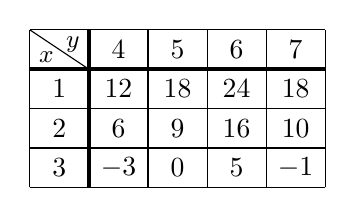
\begin{tikzpicture}[x=.75cm,y=.5cm]
      \draw (0,0) grid [step=1] (5,4);
    
      \draw[ultra thick] (0,3)--(5,3);
      \draw[ultra thick] (1,4)--(1,0);
      
      \draw (0,4) -- (1,3);
      \node at (.9,3.9) [below left,inner sep=1pt] {\small$y$};
      \node at (0.1,3.1) [above right,inner sep=1pt] {\small$x$};
      
      %% x-values
      \node at (0.5,2.5) {$1$};
      \node at (0.5,1.5) {$2$};
      \node at (0.5,0.5) {$3$};
      
      %% y-values
      \node at (1.5,3.5) {$4$};
      \node at (2.5,3.5) {$5$};
      \node at (3.5,3.5) {$6$};
      \node at (4.5,3.5) {$7$};
      
      %% z-values
      %% top row
      \node at (1.5,2.5) {$12$};
      \node at (2.5,2.5) {$18$};
      \node at (3.5,2.5) {$24$};
      \node at (4.5,2.5) {$18$};
      
      %% second row
      \node at (1.5,1.5) {$6$};
      \node at (2.5,1.5) {$9$};
      \node at (3.5,1.5) {$16$};
      \node at (4.5,1.5) {$10$};
      
      %% third row
      %% second row
      \node at (1.5,.5) {$-3$};
      \node at (2.5,.5) {$0$};
      \node at (3.5,.5) {$5$};
      \node at (4.5,.5) {$-1$};
    \end{tikzpicture}
  \end{image}
  Estimate
  \[
  F^{(1,0)}(2,6)
  \]
  \begin{explanation}
    To estimate $F^{(1,0)}(2,6)$ we examine the change between $x=1$
    and $x=2$:
    \begin{align*}
      \frac{F(2,6)-F(1,6)}{2-1}&= \frac{\answer[given]{16}-\answer[given]{24}}{2-1}\\
      &=\answer[given]{-8}
    \end{align*}
    We also should examine the change between $x=2$ and $x=3$:
    \begin{align*}
      \frac{F(3,6)-F(2,6)}{3-2}&= \frac{\answer[given]{5}-\answer[given]{16}}{3-2}\\
      &=\answer[given]{-11}
    \end{align*}
    Now if we average these values together, we see
    \[
    \eval{\pp{x} F(x,y)}_{(x,y)=(2,6)} \approx \answer[given]{-9.5}
    \]
  \end{explanation}
\end{example}

\begin{question}
  Let $F:\R^2\to\R$ be described by the following table of values:
  \begin{image}
    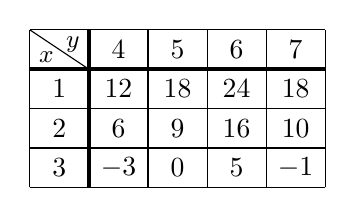
\begin{tikzpicture}[x=.75cm,y=.5cm]
      \draw (0,0) grid [step=1] (5,4);
      
      \draw[ultra thick] (0,3)--(5,3);
      \draw[ultra thick] (1,4)--(1,0);
      
      \draw (0,4) -- (1,3);
      \node at (.9,3.9) [below left,inner sep=1pt] {\small$y$};
      \node at (0.1,3.1) [above right,inner sep=1pt] {\small$x$};
      
      %% x-values
      \node at (0.5,2.5) {$1$};
      \node at (0.5,1.5) {$2$};
      \node at (0.5,0.5) {$3$};
      
      %% y-values
      \node at (1.5,3.5) {$4$};
      \node at (2.5,3.5) {$5$};
      \node at (3.5,3.5) {$6$};
      \node at (4.5,3.5) {$7$};
      
      %% z-values
      %% top row
      \node at (1.5,2.5) {$12$};
      \node at (2.5,2.5) {$18$};
      \node at (3.5,2.5) {$24$};
      \node at (4.5,2.5) {$18$};
      
      %% second row
      \node at (1.5,1.5) {$6$};
      \node at (2.5,1.5) {$9$};
      \node at (3.5,1.5) {$16$};
      \node at (4.5,1.5) {$10$};
      
      %% third row
      %% second row
      \node at (1.5,.5) {$-3$};
      \node at (2.5,.5) {$0$};
      \node at (3.5,.5) {$5$};
      \node at (4.5,.5) {$-1$};
    \end{tikzpicture}
  \end{image}
  Estimate
  \[
  F^{(0,1)}(2,6)
  \begin{prompt}
    \approx \answer{.5}
  \end{prompt}
  \]
  \begin{hint}
    Work as we did in the example above, finding two estimates and taking their averages. 
  \end{hint}
\end{question}

LEVEL CURVES ARE NEXT

  \section{Combining partial derivatives}

\end{document}
